\section{User Interface}
This section will look at how each of the designed UI aspects was implemented. UI implementation made use of controllers, which were responsible for conducting database interactions and returning relevant views, along with HTML, CSS and Javascript for page structure, design and usability. Implementation for different UI components was identical to the concept designs discussed in Chapter \ref{Chapter:Design}.

\subsection{Navigation}
Figure \ref{fig:NavImplementation} shows the implemented navigation bars for authorised users and guests. Users are able to navigate to the pages represented by each of the icons on the navigation bar. The page the user is currently on is represented by an orange underline under the corresponding icon on the navigation bar.

\begin{figure}[H]
    \centering
    \begin{subfigure}{1\linewidth}
        
\includegraphics[width=1\textwidth]{Images/Design/nav-unauthorised}
        \caption{Guest}
        \label{fig:NavUnauth}
    \end{subfigure}
    \begin{subfigure}{1\linewidth}
        
\includegraphics[width=1\textwidth]{Images/Design/nav-authorised}
        \caption{Authorised User}
        \label{fig:NavAuth}
    \end{subfigure}
    \caption{Navigation bar for (a) guests and (b) authorised users}
    \label{fig:NavImplementation}
\end{figure}

\subsubsection{Links}
Routes for each of the icons are populated using the \textit{LayoutComposer} class, which is a class method that is called whenever the Layout view is rendered \cite{Laravel:Views}. The navigation bar is rendered in the \emph{Layout} view. Depending on whether the user is authorised or not, the composer returns the title, icon name, route and CSS properties of the relevant icon. Figure \ref{fig:LayoutComposerNav} shows the navigation options for user and application navigation.

\begin{figure}[H]
\centering
\begin{subfigure}[b]{1\linewidth}
    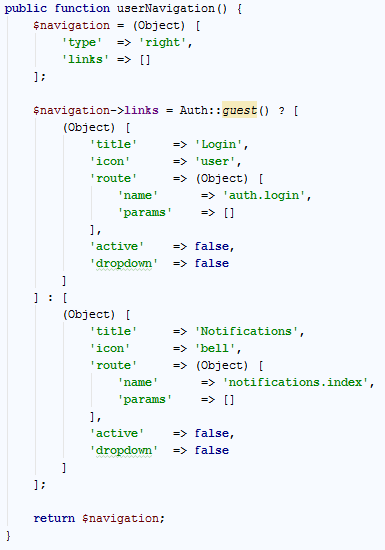
\includegraphics[width=1\textwidth]{Images/Implementation/UserNavigation}
    \caption{User navigation}
    \label{fig:UserNavigation}
\end{subfigure}
\begin{subfigure}[b]{1\linewidth}
    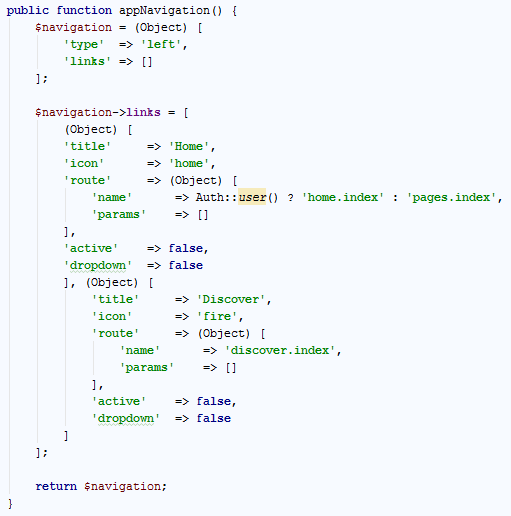
\includegraphics[width=1\textwidth]{Images/Implementation/AppNavigation}
    \caption{Application navigation}
    \label{fig:AppNavigation}
\end{subfigure}
\caption{Rendering options in \emph{LayoutComposer}}
\label{fig:LayoutComposerNav}
\end{figure}

\subsubsection{Search}
The search bar allows users to enter a query term, and any user or tag matching this search term is retrieved. Using jQuery and JSON, it is possible to live-update the results from the supplied query term and display them to the user. Doing this removes the need to re-direct the user to a separate page which displays the search results to them. An API call to the \textit{SearchController} is made, in which all users and tags matching the query term are retrieved and returned to the view as a JSON object. Figure \ref{fig:SearchController} shows the retrieval of results that match the search term.

\begin{figure}[H]
\centering
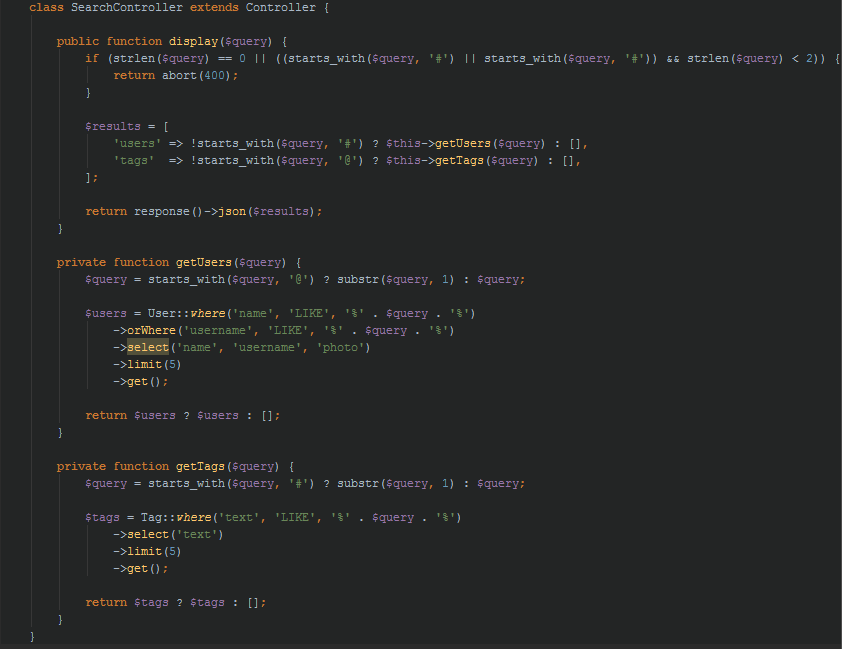
\includegraphics[width=1\textwidth]{Images/Implementation/SearchController}
\caption{Processing of query term performed in \textit{SearchController}}
\label{fig:SearchController}
\end{figure}

It is also possible to search specifically for a user or tag by preceding the query term with a \textbf{@} or \textbf{\#} symbol. Doing this restricts the results returned from the search to just users or tags. In Figure \ref{fig:SearchResults} we can see the implemented search bar, showing the results of providing `H' as a query term.

\begin{figure}[H]
\centering
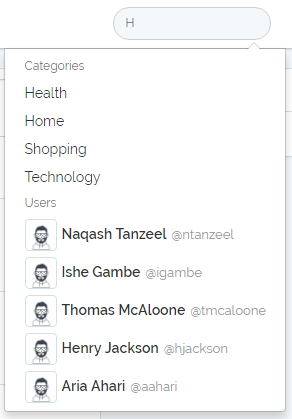
\includegraphics[height=2in]{Images/Implementation/SearchResults}
\caption{Results from searching for the term `H'}
\label{fig:SearchResults}
\end{figure}

\subsection{Authentication}
Laravel provides built-in functionality for handling user authentication. With this, a number of controllers are available that manage authentication for user login, registration and password recovery \cite{Laravel:Authentication}. By executing the \textit{php artisan make:auth} command, all views and controllers related to user authentication are generated. This command also generates the routes required to navigate to the views, and access controller functionality.

\subsubsection{Registration}
The form on the registration page, shown in Figure \ref{fig:RegisterPage}, collects the user's name, email address, username, date of birth, password, and also asks the user to agree with the Fidelis terms of service. If the user provides all the required fields, they are re-directed to the home page. The post-authentication redirect location can be modified in the \textit{RegisterController}.

\begin{figure}[H]
\centering
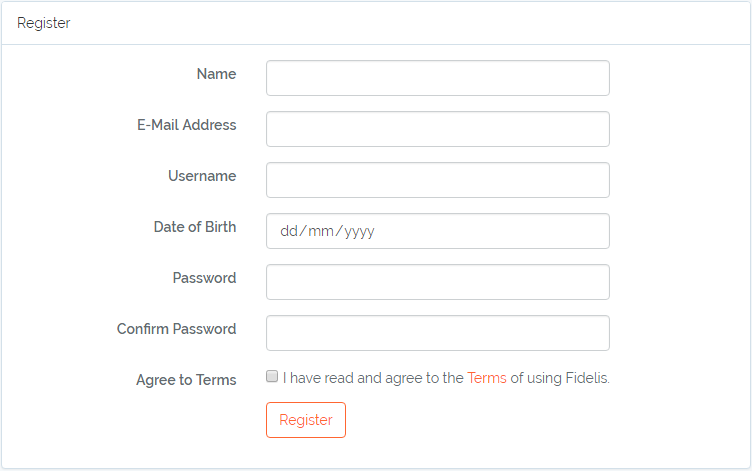
\includegraphics[height=2in]{Images/Design/register-page}
\caption{Registration page}
\label{fig:RegisterPage}
\end{figure}

In addition to the redirection location, the \textit{RegisterController} contains \textit{validator()} and \textit{create()} functions. Before the user is redirected to the home page on successful authentication, the controller first applies a set of validation rules specified in the validator (figure \ref{fig:RegValidation}) which must be verified before the user is authenticated. If validation is correct, the new user is created and authenticated (figure \ref{fig:register-controller}), leading to successful redirection. If validation is unsuccessful, an error message is displayed to the user, providing a visual prompt informing the user of what input was incorrect and should be modified.

\begin{figure}[H]
\centering
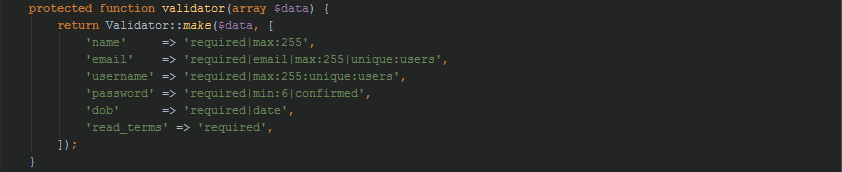
\includegraphics[width=\textwidth]{Images/Implementation/RegisterValidation}
\caption{Validation rules applies to the registration form fields}
\label{fig:RegValidation}
\end{figure}

\subsubsection{Login}
The login page, shown in Figure \ref{fig:LoginPage}, requests the user's email address and password. Similarly to registration, users who are successfully authenticated are redirected to the homepage. All authentication functionality is handled by the pre-built \textit{LoginController}. If incorrect account credentials are provided, authentication is unsuccessful. Reasons for unsuccessful authentication are displayed to the user in a similar manner as on the registration page.

\begin{figure}[H]
\centering
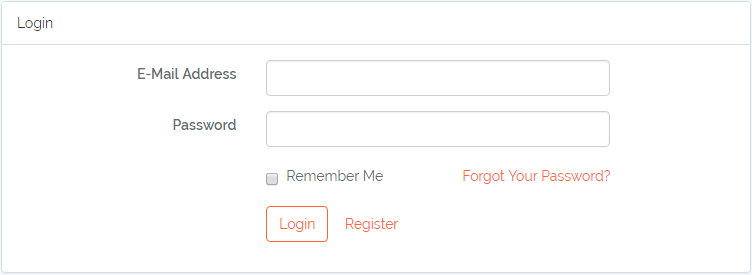
\includegraphics[height=1.5in]{Images/Design/login-page}
\caption{Log-in page}
\label{fig:LoginPage}
\end{figure}

\subsubsection{Password Reset}
The password reset page, shown in Figure \ref{fig:PasswordReset} allows users to reset their passwords if they have forgotten their account credentials. By navigating to this page, users can submit a form containing their email address. Submission of this form will prompt the \textit{ResetController}, which handles password resetting using pre-built functionality, to send a password reset link to the provided email address if an account exists for that address.

\begin{figure}[H]
\centering
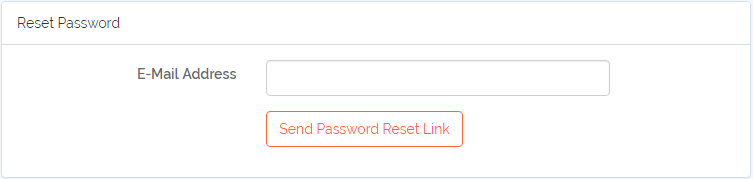
\includegraphics[height=1in]{Images/Implementation/PasswordReset}
\caption{Account recovery page}
\label{fig:PasswordReset}
\end{figure}

\subsection{Home}
The Fidelis home is the hub of the entire website. It is the first place a user will typically be directed to and will show one of two pages depending on if the user is logged into an account.

\subsubsection{Landing Page}
When a user first navigates to the Fidelis platform - either for the first time or if they are not logged into an account - they will arrive on the landing page shown in figure \ref{fig:HomeUnauthorised}.  

\begin{figure}[H]
\centering

\includegraphics[width=\textwidth]{Images/Implementation/home_unauthorised}
\caption{Landing Page}
\label{fig:HomeUnauthorised}
\end{figure}

This landing page is created by the view shown in Figure \ref{fig:LandingView}. We can see that if the user is detected to be a guest, i.e., not logged into an account, this page will be shown. The view provides two buttons at the top right of the page, one for logging into an existing account, and one for signing up for a new account. In addition, a background wallpaper will be provided randomly from a number of stored image assets. Finally the title of the website, `Fidelis', is displayed along with a quote (and a name of the person to whom the quote is attributed) regarding trust - the central theme of Fidelis.

\begin{figure}[H]
\centering
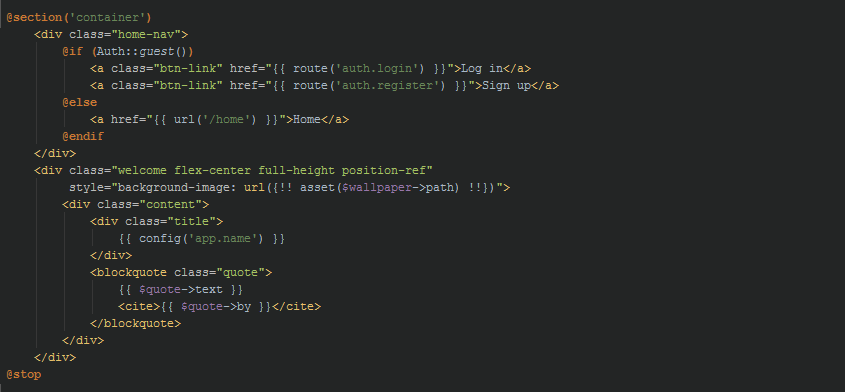
\includegraphics[width=\textwidth]{Images/Implementation/LandingView}
\caption{Landing page view}
\label{fig:LandingView}
\end{figure}

\subsubsection{Home Page}
If it is determined that the user is logged in when they navigate to the Fidelis home page, they will be routed from this landing page to the home page shown in Figure \ref{fig:HomeAuthorised}.

\begin{figure}[H]
\centering
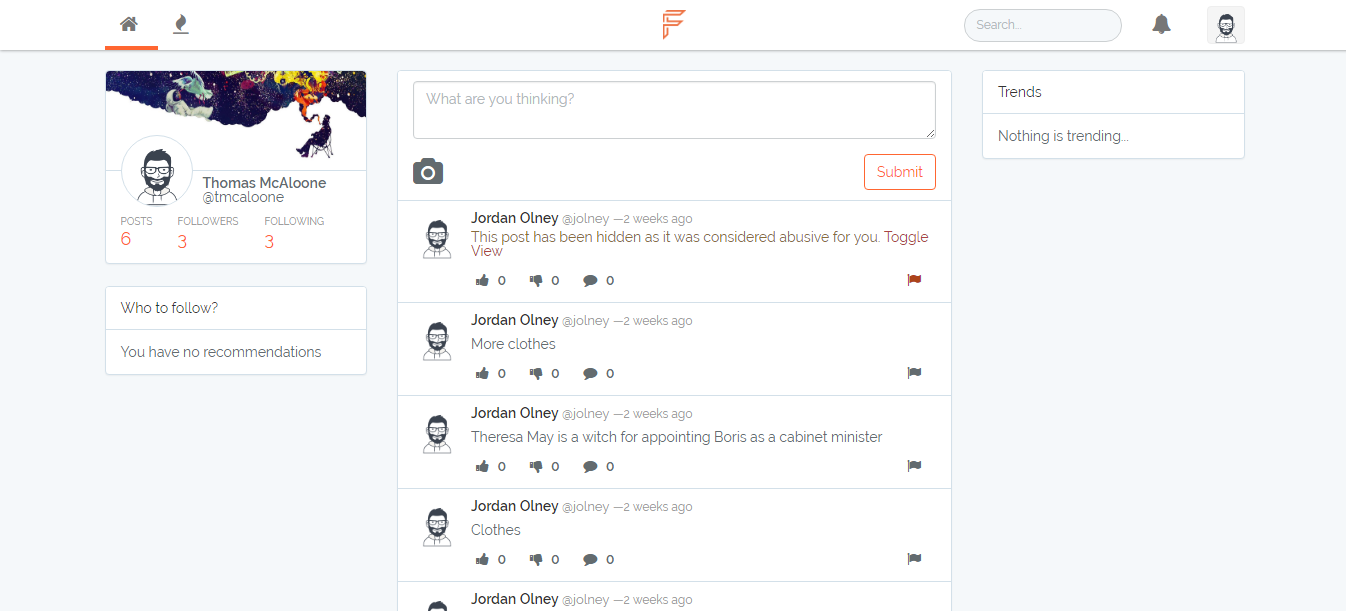
\includegraphics[width=\textwidth]{Images/Implementation/home_authorised}
\caption{Home Page}
\label{fig:HomeAuthorised}
\end{figure}

Upon the user being directed to the homepage, a call will be made to the \textit{index()} function of the \textit{HomeController} via the relevant route, as seen in figure \ref{fig:HomeRoutingController}. The \textit{index()} function is responsible for retrieving the posts made by accounts the user follows. These posts are then returned to the home page to be displayed in order from the most recent post to the oldest.

\begin{figure}[H]
\centering
\begin{subfigure}[b]{1\linewidth}
    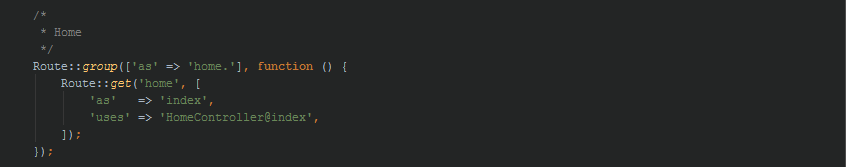
\includegraphics[width=\textwidth]{Images/Implementation/HomeRouting}
    \caption{}
    \label{fig:HomeRouting}
\end{subfigure}
\begin{subfigure}[b]{1\linewidth}
    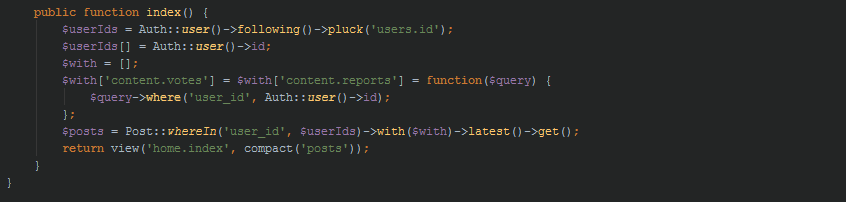
\includegraphics[width=1\textwidth]{Images/Implementation/HomeControllerIndexFunction}
    \caption{}
    \label{fig:HomeControllerIndexFunction}
\end{subfigure}
\caption{(a) Home page routing and (b) $index()$ function of the $HomeController$}
\label{fig:HomeRoutingController}
\end{figure}

Once the posts from accounts the user is following have loaded in, the user also has the ability to create and share their own content. The user can write posts by typing text into the available text area to be submitted with the post. In addition, there is an icon which can be clicked to upload a photo with the post. The form is handled using AJAX so that when the post has successfully been uploaded, the current page can be updated with that post without the need to refresh the page. If the page had to be refreshed upon every post submission the entire page would have to be loaded again, including the post feed which may then show different posts than those the user had been viewing. Using AJAX simply provides a better user experience and allows smoother interaction with the Fidelis website.

\begin{figure}[H]
\centering
\begin{subfigure}[b]{1\linewidth}
    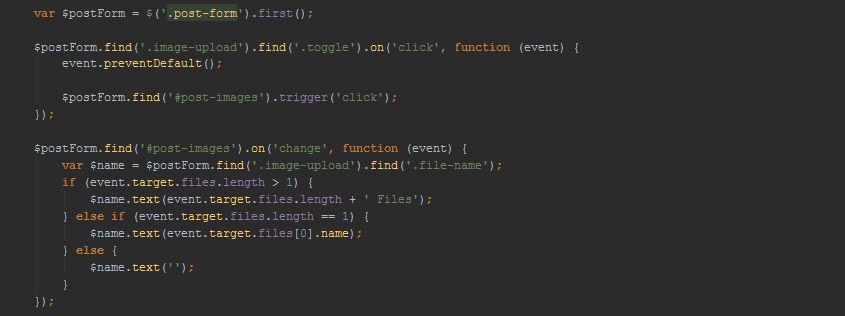
\includegraphics[width=\textwidth]{Images/Implementation/HomeNewPostJS}
    \caption{}
    \label{fig:HomeNewPostJS}
\end{subfigure}
\begin{subfigure}[b]{1\linewidth}
    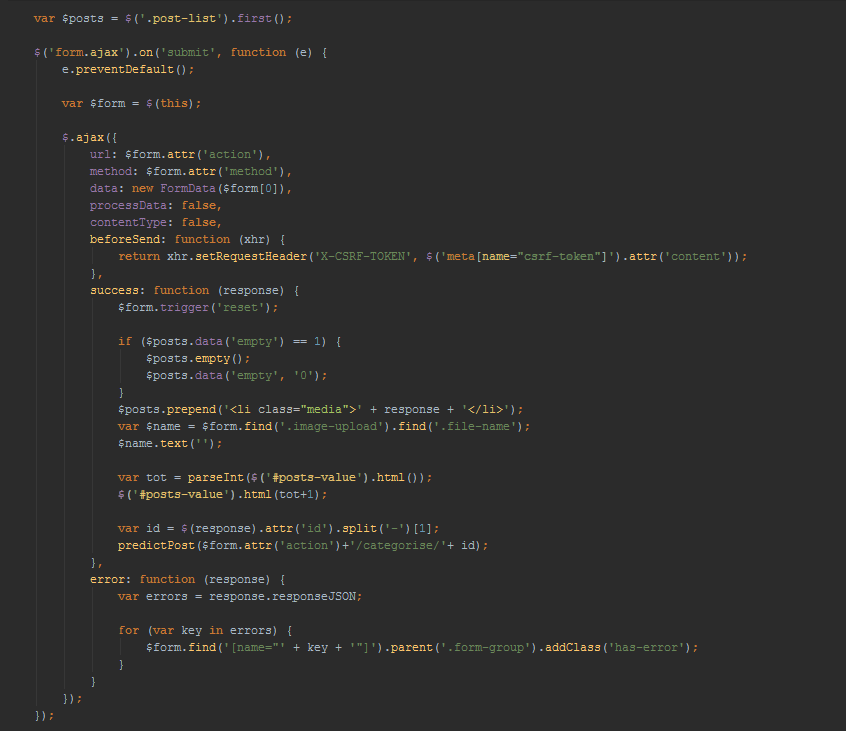
\includegraphics[width=\textwidth]{Images/Implementation/HomeNewPostJS2}
    \caption{}
    \label{fig:HomeNewPostJS2}
\end{subfigure}
\caption{Javascript code for handling a new post: (a) inserting and image and (b) submitting the form}
\label{fig:HomeNewPostJavascript}
\end{figure}

Figure \ref{fig:HomeNewPostJavascript} shows the javascript code that is used to handle image uploads, as well as the code handling the submission of the form (Once the user hits submit to create the post). At this point, the new post will be automatically categorised using the script $predict.py$. Upon submission of the form, the form will route a post request using the $store()$ function in the $PostController$. This function simply stores the new post in the database and then returns the same post to the home page. This post will then appear at the top of the post feed for the user.

In order to represent a post for the $PostContoller$, a PHP trait named $Post$ was created. This trait features a number of functions defining all of the interactions a post can have on the Fidelis platform. Figure \ref{fig:PostTrait} shows some of these functions, for example, the $add()$ function, which will save the post to the database, including any images uploaded with the post and tags on the post. Note that this function is called by the $store()$ function in the $PostController$ to store the post in the database as described previously. Figure \ref{fig:PostTrait} also shows the function $addComment()$ used to add and store a new comment on the current post and the function $notifyUsers()$ which is used to notify a user when a post of theirs is commented on, or when they have been mentioned in a post/comment.

\begin{figure}[H]
\centering
\begin{subfigure}[b]{1\linewidth}
    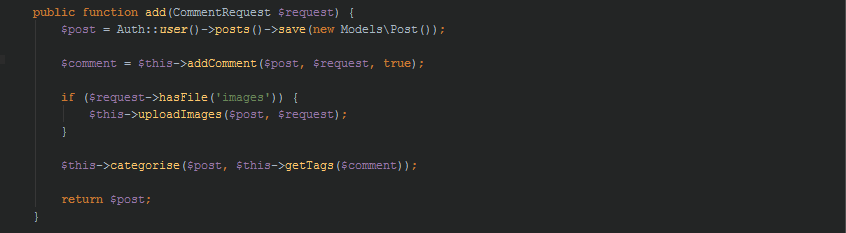
\includegraphics[width=\textwidth]{Images/Implementation/PostTraitAdd}
    \caption{}
    \label{fig:PostTraitAdd}
\end{subfigure}
\begin{subfigure}[b]{1\linewidth}
    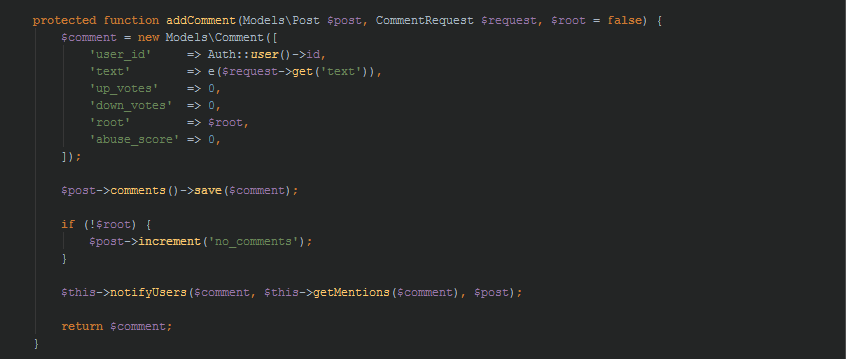
\includegraphics[width=\textwidth]{Images/Implementation/PostTraitAddComment}
    \caption{}
    \label{fig:PostTraitAddComment}
\end{subfigure}
\begin{subfigure}[b]{1\linewidth}
    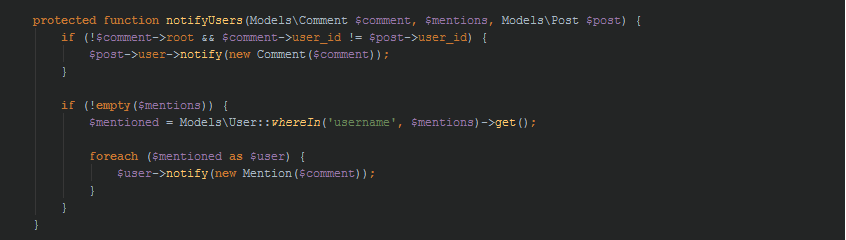
\includegraphics[width=\textwidth]{Images/Implementation/PostTraitNotifyUsers}
    \caption{}
    \label{fig:PostTraitNotifyUsers}
\end{subfigure}
\caption{Post trait example functions: (a) Add this post to database, (b) Add new comment to this post and (c) Notify users about comments on this post}
\label{fig:PostTrait}
\end{figure}

In addition to the functions show in Figure \ref{fig:PostTrait}, a number of other functions are present in the $Post$ trait, including: $getMentions()$, which returns any users mentioned in a post/comment; $uploadImages()$, which takes any images uploaded on a post and stores them in the database; $getNonTags()$, which generates tags from words in a post; $categorise()$, which will store any tags from a post, or, if non exist, will call the $getNonTags()$ function to generate tags from words in the post, where there an existing a tag in the database for those words; and finally, $getTags()$, which finds any tags on a post.

\subsection{Discover}
The implemented discover page is shown in Figure \ref{fig:DiscoverPage}. This page gives the ability for a user to seek out and find new content, which appeals to them, outside of the content they see from their current network. The user can use this page to find new content from specific categories, see content from tags they have subscribed to and manage their subscriptions, as well as seeing content recommended for them.

\begin{figure}[H]
\centering
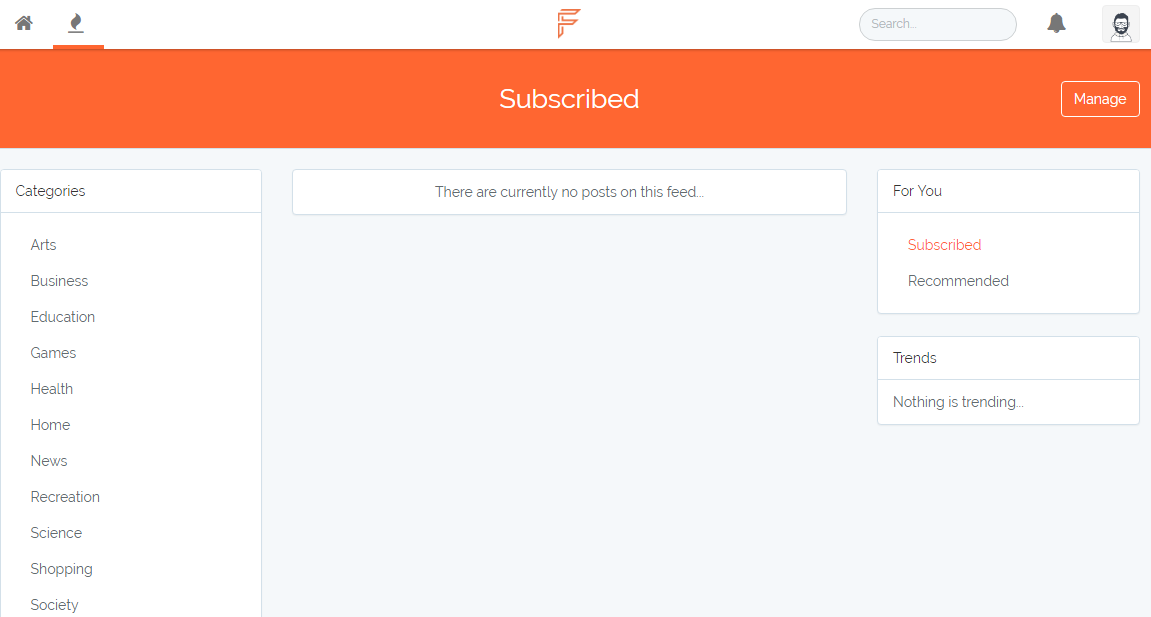
\includegraphics[width=\textwidth]{Images/Implementation/DiscoverPage}
\caption{Discover Page}
\label{fig:DiscoverPage}
\end{figure}

The banner seen across the top of the page contains the title of the current page. The title that is shown therefore depends on which data is being displayed. For each case, a separate view has been created to display the correct title. This is usually the name of the category, however, there are exceptions for viewing the user's subscriptions - in which case a button must also be included to link to the Settings page where the user can manage their subscriptions - as well as viewing the user's recommended content. Figure \ref{fig:DiscoverTitle} shows these different views.

\begin{figure}[H]
\centering
\begin{subfigure}[b]{1\linewidth}
    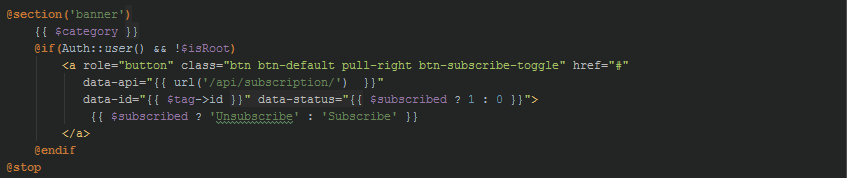
\includegraphics[width=\textwidth]{Images/Implementation/CategoryBladePhp}
    \caption{}
    \label{fig:CategoryBladePhp}
\end{subfigure}
\begin{subfigure}[b]{1\linewidth}
    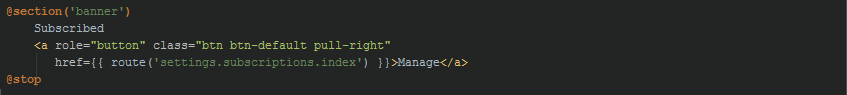
\includegraphics[width=\textwidth]{Images/Implementation/IndexBladePhp}
    \caption{}
    \label{fig:IndexBladePhp}
\end{subfigure}
\begin{subfigure}[b]{1\linewidth}
    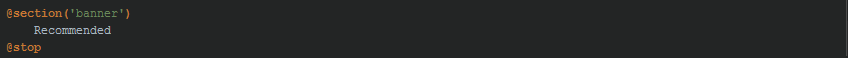
\includegraphics[width=\textwidth]{Images/Implementation/RecommendedBladePhp}
    \caption{}
    \label{fig:RecommendedBladePhp}
\end{subfigure}
\caption{Different view outputs of Title for (a) Categories, (b) Subscribtions and (c) Recommendations}
\label{fig:DiscoverTitle}
\end{figure}

In order to determine which content needs to be loaded to the post feed, the system determines which option is `active', i.e., whether the user has selected to view content they are subscribed to, content recommended for them, or content from a category. For each of these options, there is a corresponding route to follow. These routes are shown in figure \ref{fig:DiscoverRouting}.

\begin{figure}[H]
\centering
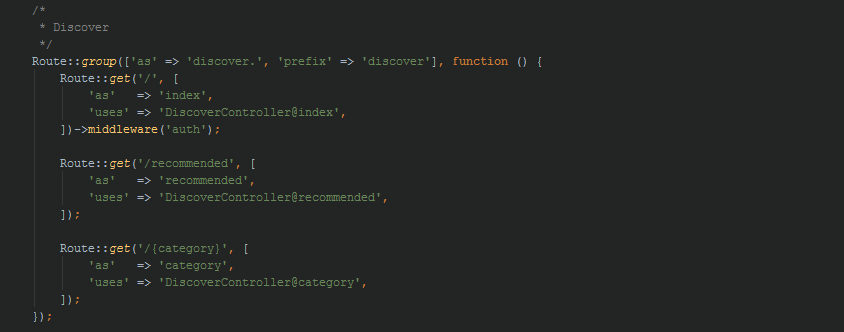
\includegraphics[width=\textwidth]{Images/Implementation/DiscoverRouting}
\caption{Discover Routing}
\label{fig:DiscoverRouting}
\end{figure}

\subsubsection{Discover Controller Actions}
Each of the routes followed from the discover page result in a different action being taken by the \textit{DiscoverController}. Note that routing to the index route for subscriptions here requires a check to ensure the user is authorised to take that action as a guest will have no subscriptions. Each of these actions will ultimately return a number of posts from the database to be handled by the discover page.

\paragraph{Subscribed Content}
The $index()$ function of the $Discover  Controller$ is shown in figure \ref{fig:DiscoverControllerSubscribed}. This function will call the $subscriptions()$ relation of the $User$ model, shown in Figure \ref{fig:SubscribedPosts}. The $subscriptions()$ relation returns all of the subscriptions a user has. The id of every tag the user is subscribed to will then be retrieved. The function then collects every post that has a tag, where the user is subscribed to that tag. These posts are then returned to the discover page to be displayed in order from the most recent to the oldest post.

\begin{figure}[H]
\centering
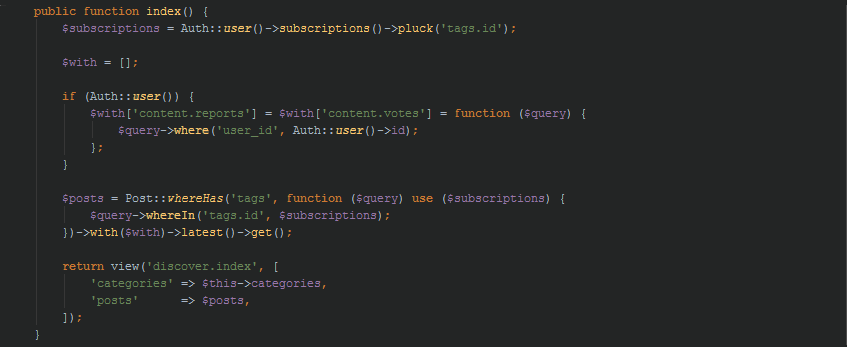
\includegraphics[width=\textwidth]{Images/Implementation/DiscoverControllerSubscribed}
\caption{Discover Controller action for displaying subscribed content}
\label{fig:DiscoverControllerSubscribed}
\end{figure}

\begin{figure}[H]
\centering
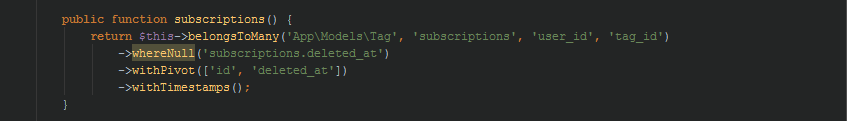
\includegraphics[width=\textwidth]{Images/Implementation/SubscribedPosts}
\caption{$subscriptions()$ relation}
\label{fig:SubscribedPosts}
\end{figure}

\paragraph{Recommended Content}
The $recommend()$ function of the $Discover  Controller$ is shown in Figure \ref{fig:DiscoverControllerSubscribed}. This function will call the $recommendedPosts()$ relation of the $User$ model shown in Figure \ref{fig:RecommendedPosts}. The $recommendedPosts()$ relation simply returns all posts that are recommended to the given user. These posts are then returned to the discover page to be displayed in order from the most recent to the oldest post.

\begin{figure}[H]
\centering
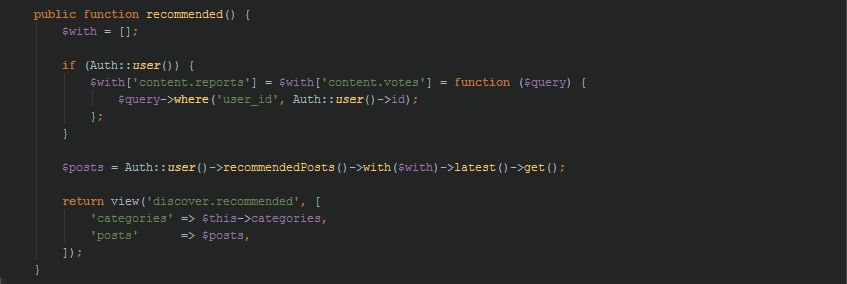
\includegraphics[width=\textwidth]{Images/Implementation/DiscoverControllerRecommended}
\caption{Discover Controller action for displaying recommended content }
\label{fig:DiscoverControllerRecommended}
\end{figure}

\begin{figure}[H]
\centering
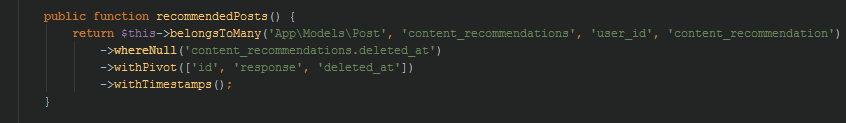
\includegraphics[width=\textwidth]{Images/Implementation/RecommendedPosts}
\caption{$recommendedPosts()$ relation}
\label{fig:RecommendedPosts}
\end{figure}

\paragraph{Category Content}
The $category()$ function of the $Discover  Controller$ is shown in Figure \ref{fig:DiscoverControllerSubscribed}. This function performs a few checks including finding if the $\$category$ variable passed is, in fact, a category (root tag) or simply a tag belonging to a category. This is because this function is also accessed when the user is routed to the discover page from a trending tag. If it is a root category, the function will find the id of every tag within that category and then find every post with a tag that has a matching tag id. Alternatively, if the variable passed is simply a tag belonging to a category, the function will find all posts using that tag. Either way, these posts are then returned to the discover page to be displayed in order from the most recent to the oldest post.

\begin{figure}[H]
\centering
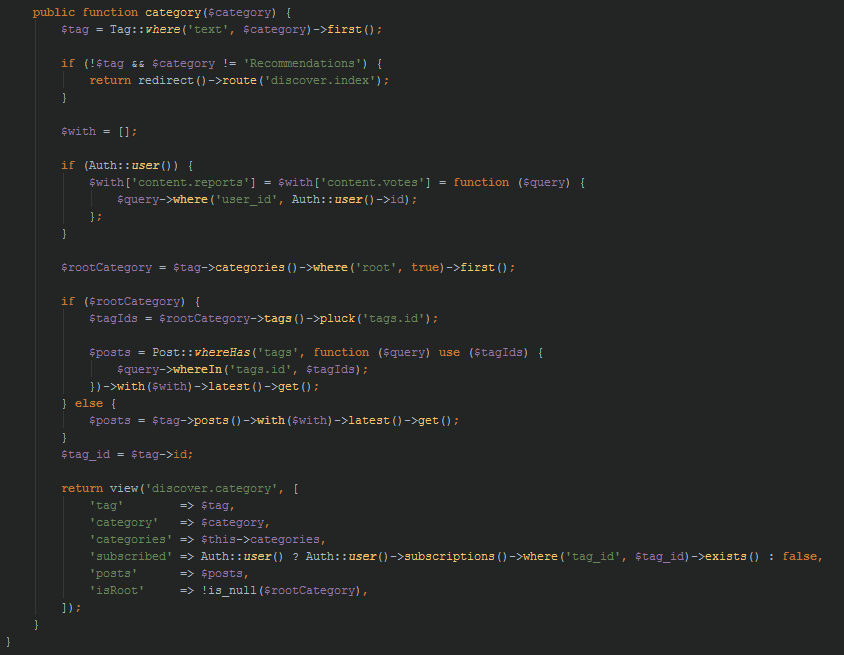
\includegraphics[width=\textwidth]{Images/Implementation/DiscoverControllerCategory}
\caption{Discover Controller action for displaying content from a category}
\label{fig:DiscoverControllerCategory}
\end{figure}

\subsection{Notifications}
Figure \ref{fig:NotificationsPage} shows the implemented notifications page. Users are notified whenever they receive a new follow, are mentioned in a post by another user, or one of their posts is commented or voted on. The page provides users with information on the notification type, and if relevant the content of the notification (for example, the comment made on their post). The counter, seen next to the bell icon on the navigation bar, indicates to the user how many unread notifications they have. The notification page only fetches unread notifications, which reduces the amount of data that is retrieved from the database. This speeds up the load time of the page. When the user visits the notifications page, all unread notifications are marked as read. 

\begin{figure}[H]
\centering
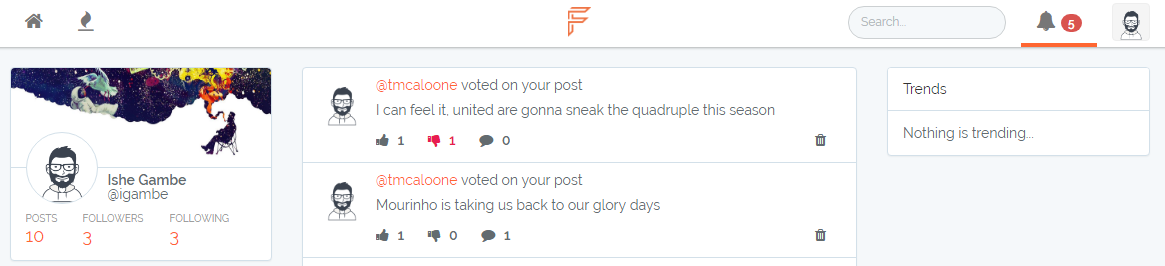
\includegraphics[width=\textwidth]{Images/Implementation/NotificationsPage}
\caption{Notifications Page}
\label{fig:NotificationsPage}
\end{figure}

Laravel provides support for integrating a notification system within your application \cite{Laravel:Notifications}. With this, it is possible to create different notification types, and have these related to a user by using the \textit{Notification} facade. Using this facade means that whenever an interaction happens with a user or with their posts, they can be notified of this using the \textit{notify()} function:

\begin{lstlisting}[language=bash]
    $user->notify(new NameOfNotification($notification)
\end{lstlisting}

Using this facade, it is also possible to queue notifications. Creating a queue of notifications can speed up application response time as there can be delays when delivering notifications to the user \cite{Laravel:Notifications, Laravel:Queues}. Queueing can be enabled by adding the \textit{Queueable} trait to the notification class, and starting a queue worker by configuring the queue in \textit{config/queue.php}. Figure \ref{fig:CommentNotification} shows the notification class created for comments. The \textit{toArray()} function contains an array that represents information carried by the notification. In the array, we have a `regarding' entry, which represents the item the notification is related to, a `to' entry which represents who the notification is meant for, and a `text' field which contains information displayed to the user receiving the notification. The fields included in each array vary depending on the type of notification.

\begin{figure}[H]
\centering
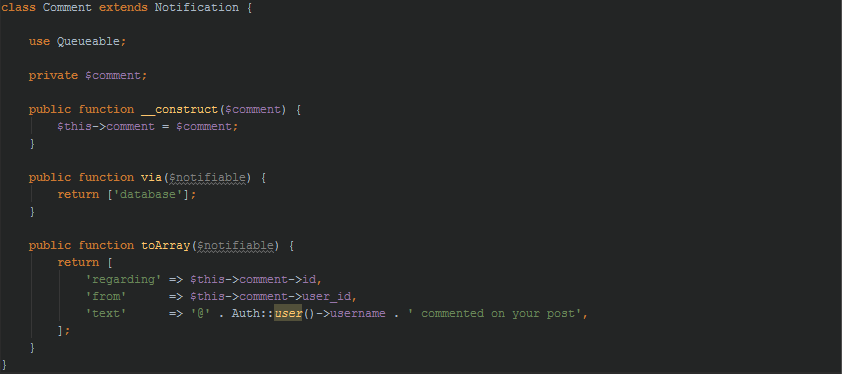
\includegraphics[width=\textwidth]{Images/Implementation/CommentNotification}
\caption{Custom notification for comments}
\label{fig:CommentNotification}
\end{figure}

\subsection{Profile}
The user profile page, shown in Figure \ref{fig:ProfilePage}, allows the user to see all their activity and public information related to their account, as well as reviewing their posts, followers and so on. A user can also view the profiles of other users which creates yet another avenue for discovering new content, as well as nurturing user-to-user interactions across the platform. Upon loading a user's profile page, their cover photo and profile picture will be loaded from the database. On the right of the page, there is also a button allowing the user to follow or unfollow the user who's page is being viewed, as well as the option to block that user. There is also a widget to the right of the page displaying trending topics.

The Follow/Unfollow button is handled by the $FollowersController$. When the button is clicked the $store()$ function is called, which will update the database to show that either the user is now following the user who owns the page, or that they are no longer than the user who owns the page. The only stipulation on this is if the user who owns the page has their account set to private. In this case, a user can only follow that user if it is a mutual relationship, i.e. they already follow that user back. The database is updated to reflect this change through the $User$ model by updating the $following()$ relation.

Alternatively, the user can decide to block the user who owns the page using the drop down arrow next to the Follow/Unfollow button. In this case, the $BlockedController$ removes any following relationships between the two users (either or both users following each other). Then the $blocked()$ relation on the $User$ model is updated to show that this user is now blocked.

\begin{figure}[H]
\centering
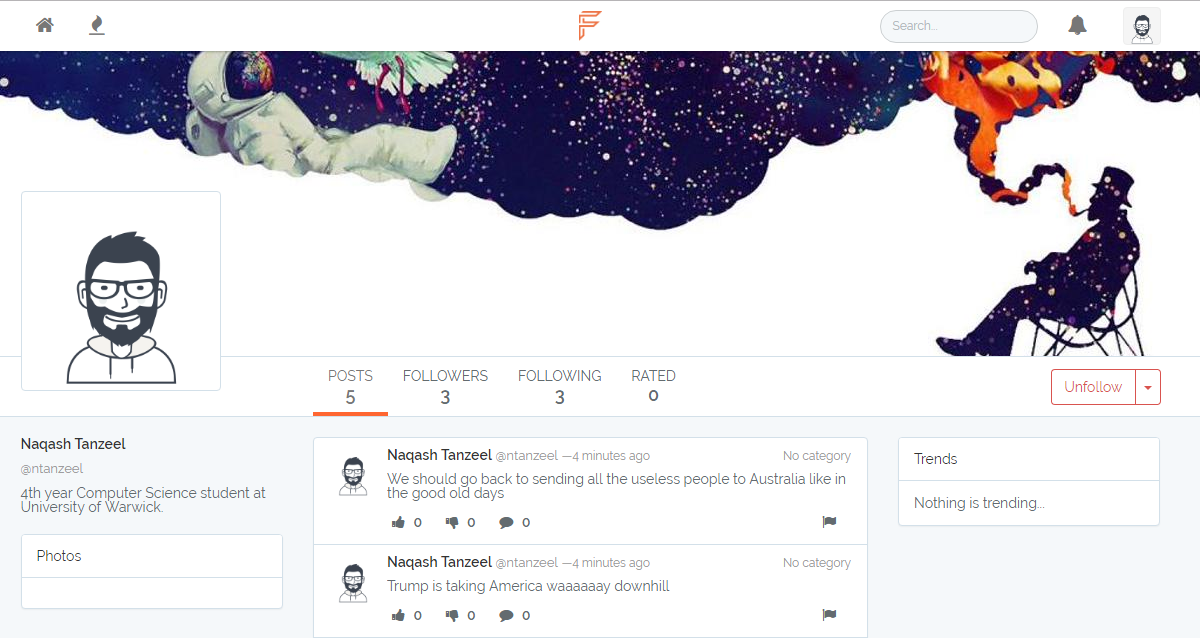
\includegraphics[width=\textwidth]{Images/Implementation/ProfilePage}
\caption{User profile page}
\label{fig:ProfilePage}
\end{figure}

If the page being viewed belongs to the user, rather than having the option to follow/unfollow/block the user, the user is instead given the option to Edit their profile. This simply links to the user's settings page. In addition, when viewing their own page a user can click an icon on their profile/cover picture to upload an image to replace their current picture. This icon is shown in Figure \ref{fig:ProfilePicUpload}. This will open a menu allowing the user to upload an image, which will then be used by the $AccountController$ to update the $User$ model and save the image to the database.

\begin{figure}[H]
\centering

\includegraphics[width=0.3\textwidth]{Images/Implementation/ProfilePicUpload}
\caption{User profile picture upload icon}
\label{fig:ProfilePicUpload}
\end{figure}

The reputation of a given user is visualised on this page in one of two ways, depending on the settings of the user viewing the page. On the settings page a used can choose to set their reputation display to either `Bar' or `Stars' in the network settings section. In order to decide which of these displays to load, the $User$ model is consulted to find the setting that this user has set for reputation display. Figure \ref{fig:ReputationRatings} shows the two displays for user reputation. In order to decide which of these displays to load, the $User$ model is consulted to find the setting that this user has set for reputation display. Firstly we have a bar which displays the user's reputation as a fraction of the highest reputation in the system (100). The bar displayed is a bootstrap component which uses the page user's reputation to set the size of the bar. We also have the star display, which again takes the user's reputation and uses it to generate a star rating out of 5, a fairly universal rating system online today. The star rating is displayed using two images, the first a background row of grey stars which are overlapped by the second image, a row of gold stars. The user reputation is used to determine how many stars are to be displayed. The front image is then cropped accordingly to give the effect that only that number of stars are `filled'. This process is handled using a jquery function when the profile page is first loaded.

\begin{figure}[H]
\centering
\begin{subfigure}[b]{.4\linewidth}
	
\includegraphics[height=1.5in]{Images/Implementation/RatingBar}
	\caption{}
	\label{fig:RatingBar}
\end{subfigure}
\begin{subfigure}[b]{.5\linewidth}
	\centering
	
\includegraphics[height=1.5in]{Images/Implementation/RatingStars}
	\caption{}
	\label{fig:RatingStars}
\end{subfigure}
\caption{Rating displays: (a) Bar display and (b) Stars display}
\label{fig:ReputationRatings}
\end{figure}

\subsubsection{User activity}
The main feature of this page is the ability to view the activity of this user. This can be done using the 4 tabs in the centre of the page: Posts, Followers, Following and Rated. Each one routes to its own page, each calling upon a different function from the \(ProfileController\).

The posts tab, shown in Figure \ref{fig:ProfilePosts}, is used to view any posts belonging to the user who's profile is being viewed. This tab calls upon the from the \(ProfileController\) function \(view()\). This function, as with each of the functions called by routes on this page, begins by calling the \(preRoute()\) function, which assesses whether the current user is authorised to view this data. Once this is confirmed, the function will find all of the posts from the user whose page is being viewed and return them ordered by the date the post was created.

\begin{figure}[H]
\centering
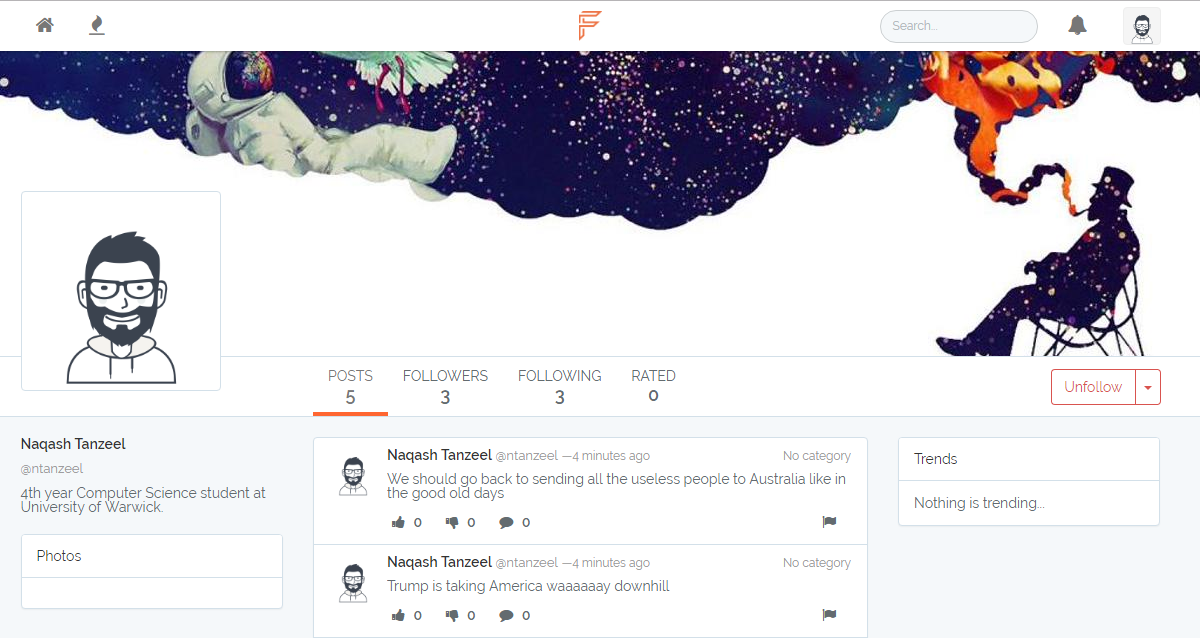
\includegraphics[width=\textwidth]{Images/Implementation/ProfilePosts}
\caption{Posts tab on the user profile page}
\label{fig:ProfilePosts}
\end{figure}

When the followers tab is selected (Figure \ref{fig:ProfileFollowers}), the \(followers()\) function from the \(ProfileController\) is called. This function firstly uses the \(preRoute()\) function, to assess whether the current user is authorised to view this data. Once this is confirmed, the \(followers()\) function will find and return all of the users who follow the user in question. These will then be displayed as a series of user widgets, one for each user following the user to whom the profile belongs. The posts are displayed in a post feed.

\begin{figure}[H]
\centering
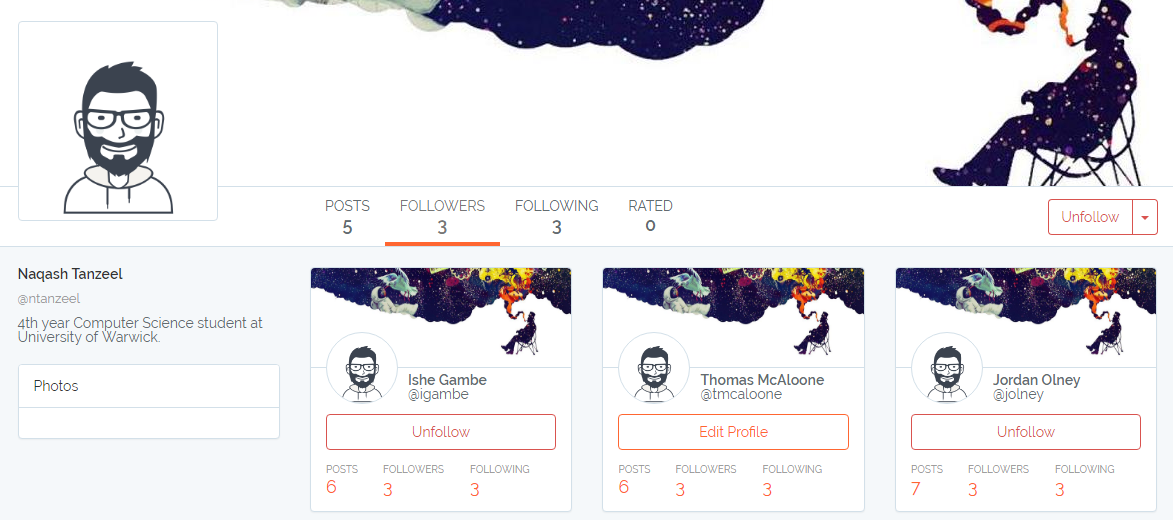
\includegraphics[width=\textwidth]{Images/Implementation/ProfileFollowers}
\caption{Followers tab on the user profile page}
\label{fig:ProfileFollowers}
\end{figure}

The following tab works in much the same way as the followers tab, however, in this case, the users that are followed by this user are shown. The \(following()\) function firstly uses the \(preRoute()\) function, to assess whether the current user is authorised to view this data. Once this is confirmed, the \(following()\) function will find and return all of the users who are followed by the user in question. These will then be displayed as a series of user widgets.

\begin{figure}[H]
\centering
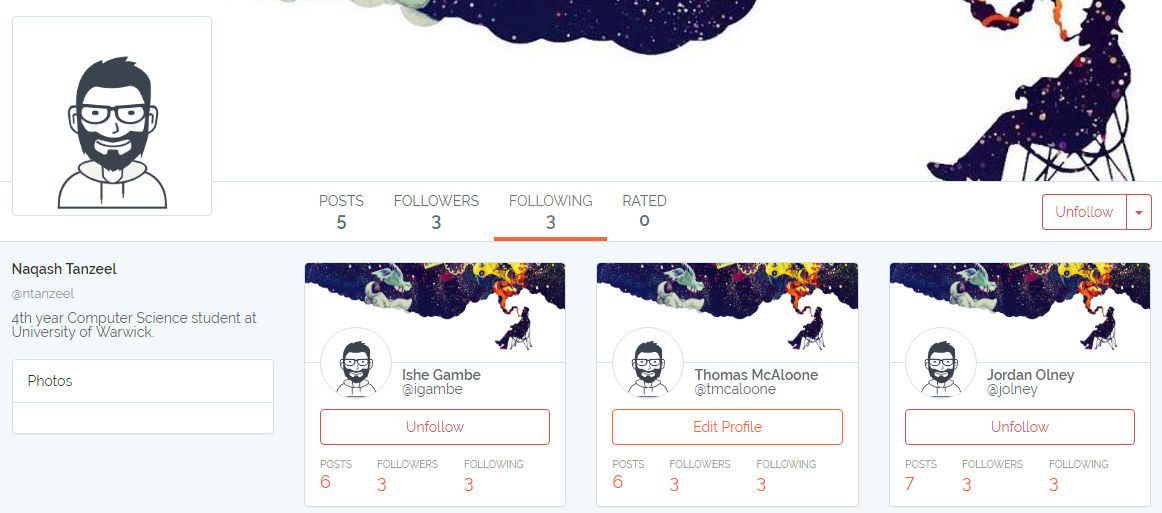
\includegraphics[width=\textwidth]{Images/Implementation/ProfileFollowing}
\caption{Following tab on the user profile page}
\label{fig:ProfileFollowing}
\end{figure}

The Rated tab displays all of the posts which this user has rated. Here `rated' simply means that the user has either upvoted or downvoted the post. The \(rated()\) function firstly uses the \(preRoute()\) function, to assess whether the current user is authorised to view this data. Once this is confirmed, the \(rated()\) function will find and return all of the posts which the user in question has rated, i.e., has either voted up or voted down. These posts are returned in order from the most recent post to the oldest post by this user. The posts are displayed in a post feed.

\begin{figure}[H]
\centering
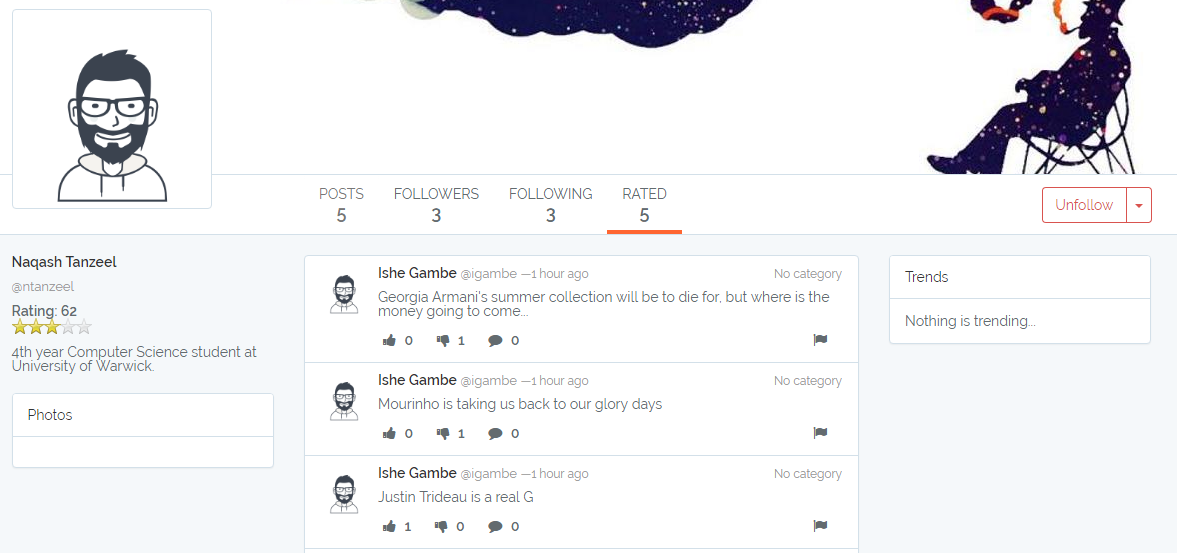
\includegraphics[width=\textwidth]{Images/Implementation/ProfileRated}
\caption{Rated tab on the user profile page}
\label{fig:ProfileRated}
\end{figure}

\subsubsection{Photos Widget}
The photos widget can be seen on the left-hand side of a user's profile page. This widget displays photos that a user has uploaded to the Fidelis Platform. Upon the page being loaded, this widget will be populated with the user's photos, retrieved from the database. The images not only appear in the widget but upon clicking one of the photos, a modal lightbox will popup over the page. The user can use this to look through all of the photos that the user has uploaded.

\subsection{Settings}
Figure \ref{fig:SettingsImplementation} shows the settings page that allows the user to toggle user account settings. The user is able to modify profile and privacy \& safety settings. In addition to this, they can also manage tags they are subscribed to, and user accounts they have blocked.

\begin{figure}[H]
\centering
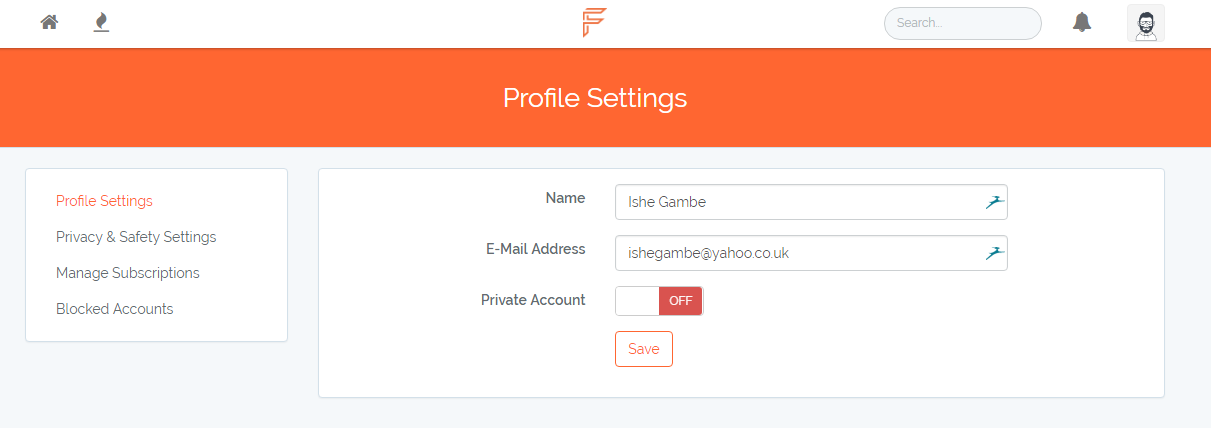
\includegraphics[width=\textwidth]{Images/Implementation/SettingsPage}
\caption{Profile settings from the settings page}
\label{fig:SettingsImplementation}
\end{figure}

Each subset of settings is handled by different controllers. The \textit{AccountController} handles any changes made by the user to their name, email address or the privacy of the account. The controller also handles requests made by the user to edit or upload their profile pictures. The \textit{SafetyController}, seen in Figure \ref{fig:SafetyController}, retrieves the user's default settings. As mentioned previously, users are able to modify settings related to abuse detection and recommendations. Before a user has had the chance to modify these settings, default settings are provided for each user. Default settings are retrieved using the query shown in figure \ref{fig:UserDefaultSettings}. The query retrieves default or custom settings by checking whether the user exists in the \emph{settings} table, before returning the relevant set of settings. This query is included as a relation on the \emph{User} model.

\begin{figure}[H]
\centering
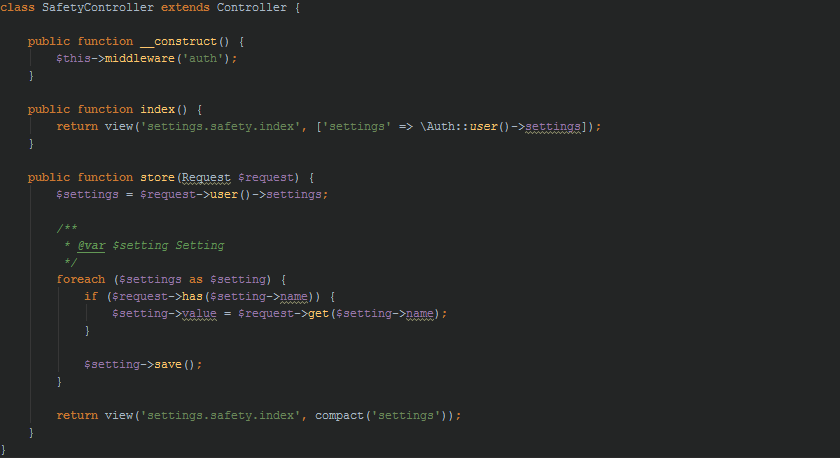
\includegraphics[width=\textwidth]{Images/Implementation/SafetyController}
\caption{Safety Controller}
\label{fig:SafetyController}
\end{figure}

The \textit{SubscriptionsController} returns the user's subscriptions in a similar fashion to how default settings are retrieved. The \textit{BlockedController} also follows this approach, using a defined relation defined on the \emph{User} model to retrieve blocked users.

\begin{figure}[H]
\centering
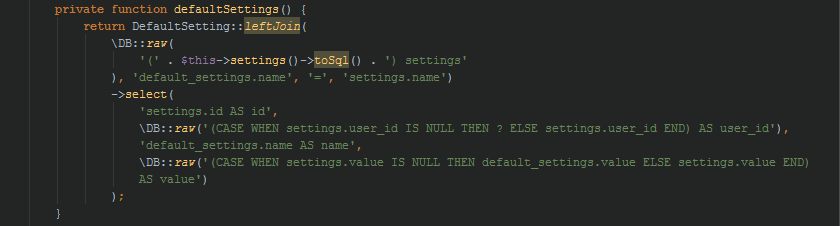
\includegraphics[width=\textwidth]{Images/Implementation/UserDefaultSettings}
\caption{Query to retrieve default settings for the user}
\label{fig:UserDefaultSettings}
\end{figure}

\subsection{Static Pages}
The two static pages aim to address the possible issues discussed in section \ref{Chapter:Issues}, by displaying information about the terms of use for Fidelis and providing support in order to help alleviate any personal issues which can arise through the use of social networking sites. These pages are accessible to both authorised users and guests visiting Fidelis. Both static pages are accessible via links in the footer.

\subsubsection{Support}
The support page displays details of how to deal with content on the site which may distress the user. Fidelis aims to keep this content to a minimum, through abuse detection, reputation scoring and terms of service. However, some content may still be posted on the platform which these measures fail to prevent. Therefore, the page lists options of how to remove the content, either by reporting it or adjusting abuse detection settings. It also provides contact details to the Samaritans \cite{Samaritans:Home}, who can offer support in case of any social issues which may arise on the network such as cyber-bullying. As seen in figure \ref{fig:SupportPage}, the styling for the page is simplistic, using bullet points in order to break down the information being provided.

\begin{figure}[H]
\centering
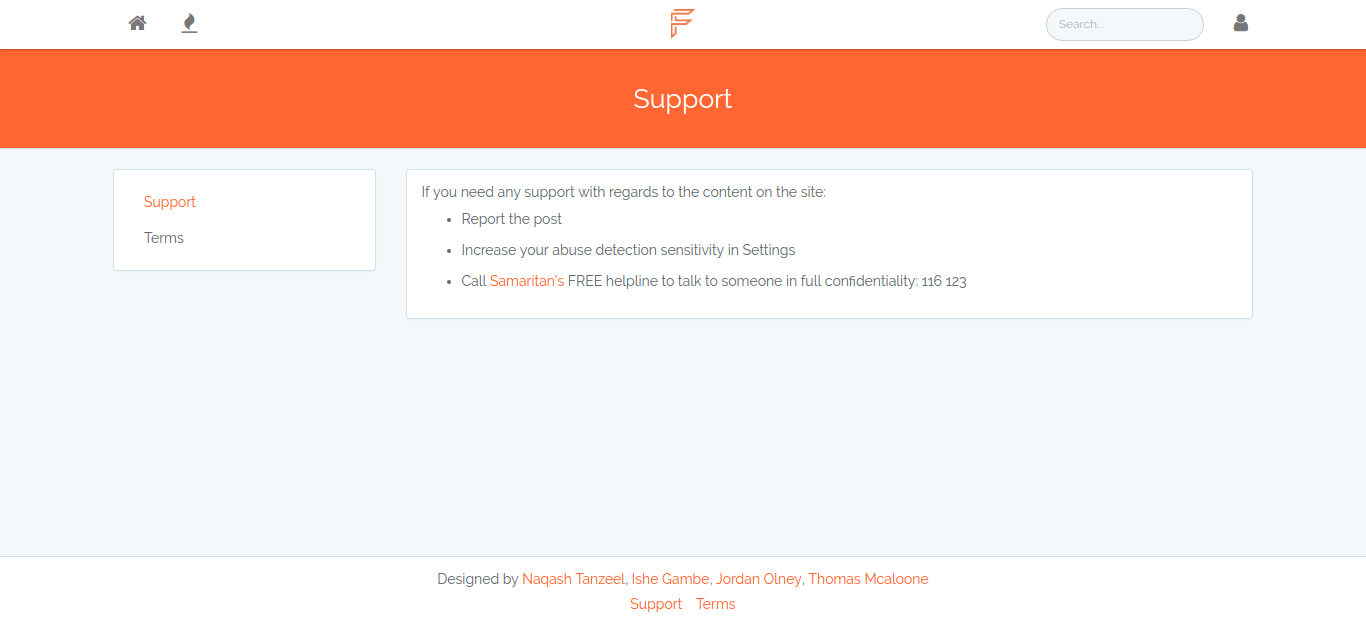
\includegraphics[width=\linewidth]{Images/Design/support-page}
\caption{Design for support page}
\label{fig:SupportPage}
\end{figure}

\subsubsection{Privacy Policy}
The styling for the terms page is the same as the support page, using bullet points to help make the information more readable, as shown in figure \ref{fig:ToS}. The information provided, however, is regarding the terms of service to ensure that the user understands what is expected of them when using the site, and the service Fidelis is expected to provide. This is to help avoid any legal issues which may arise from the content which is posted on the site by users. The Fidelis terms of service were modelled after the Twitter Private Policy \cite{Twitter:PrivatePolicy} and Terms of Service \cite{Twitter:ToS}.

\begin{figure}[H]
\centering
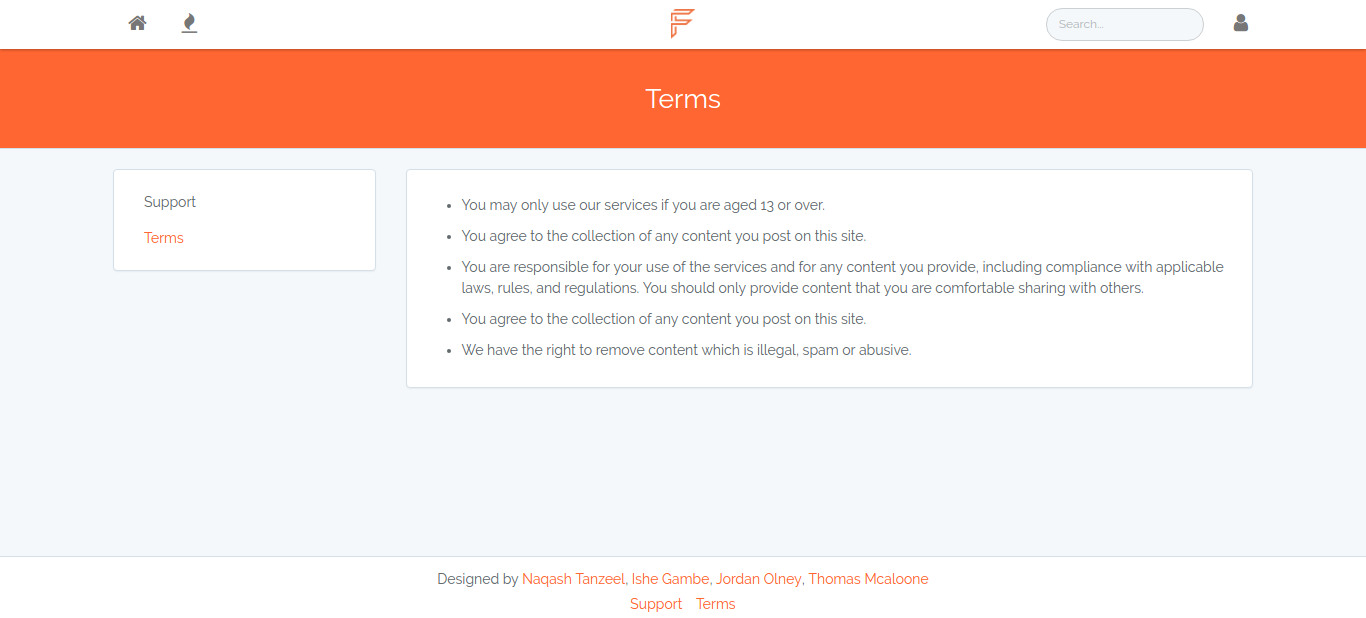
\includegraphics[width=\linewidth]{Images/Design/terms-page}
\caption{Design for terms page}
\label{fig:ToS}
\end{figure}

\subsection{Widgets}
A public Github repository created by user \textit{arrilot} provides functionality for integrating widgets into a Laravel application \cite{Packagist:LaravelWidgets}. The widget service provider available from this is ``a powerful alternative to view composers'', and as such using widgets is very similar to normal Laravel views. Widgets are standalone components which are composed of a class and a view. The class is responsible for all the logic and data for the widget and the view is responsible for displaying this data. To use these widgets, they must first be installed by running the following command:

\begin{lstlisting}[language=php]
 composer require arrilot/laravel-widgets
\end{lstlisting}

Once installed, the \textit{app.php} configuration must be updated with the registration of the new service provider. Widgets can be created in a similar fashion to controllers by using the Artisan utility:

\begin{lstlisting}[language=php]
 PHP artisan make:widget WidgetName
\end{lstlisting}

This command creates the relevant view and class for the widget. At this stage, widgets can be treated as a regular view, and can be included in existing views by using the \textit{@widget(`WidgetName')} directive. Parameters may optionally be passed to widgets and can be accessed in the \textit{run()} function of the class.

\subsubsection{Profile}
The profile widget is a standalone component that displays the profile information for a specified user, passed through as the second argument of the \textit{@widget()} directive. This widget is used on two separate pages: the home page, for displaying the logged in user's profile, and the followers/following page, for displaying the profiles of other users. These can be seen in figure \ref{fig:ProfileWidget}. The former is relatively simple as it uses a view to render the user's details. The latter, however, uses slightly more complex procedures for the following/unfollowing button. This button is rendered as a partial as it is also used on the profile page.

\begin{figure}[H]
    \centering
    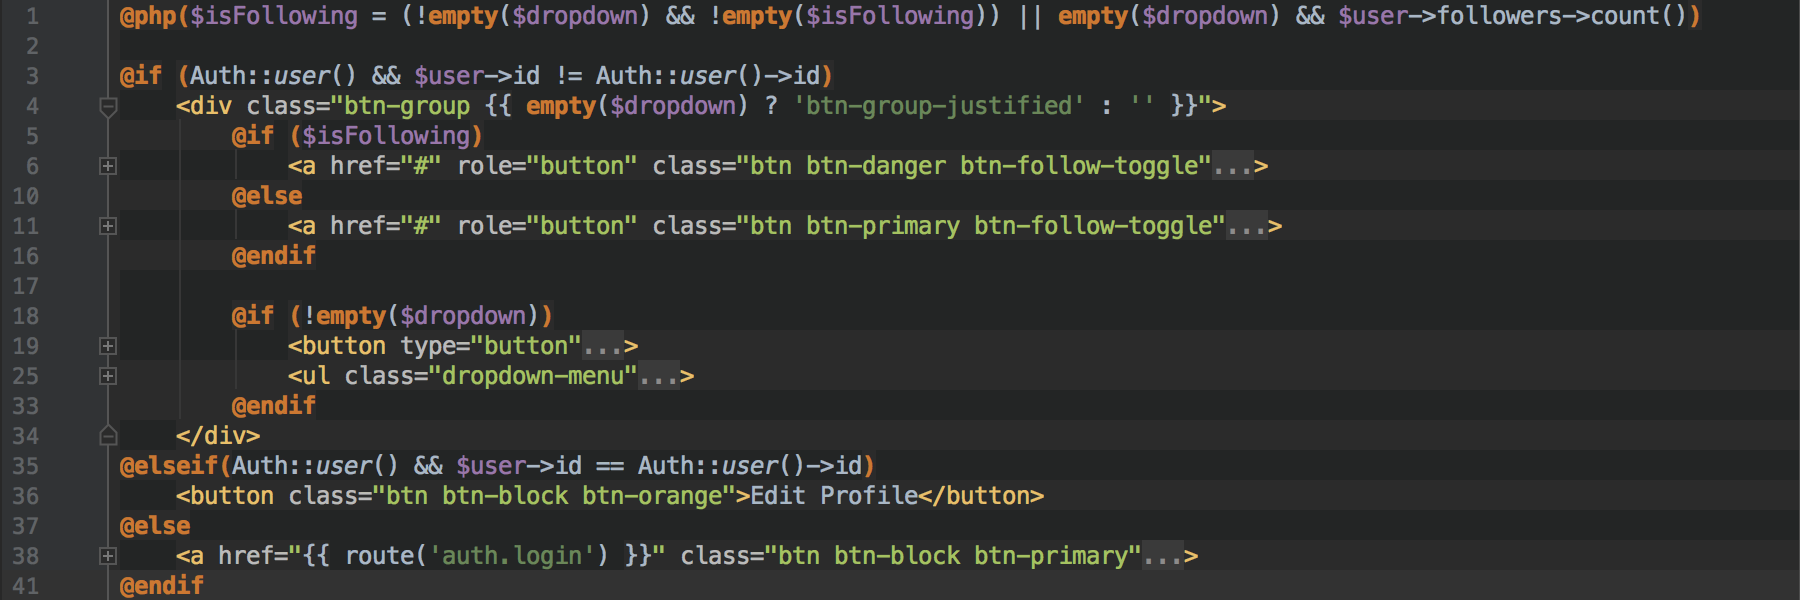
\includegraphics[width=\textwidth]{Images/Implementation/UI/Widgets/Profile_Follow}
    \caption{Code for switching the interactive button on the profile widget}
    \label{fig:Profile_Follow}
\end{figure}

In order to display the button, we need to first determine the current relationship between the users. This is done using the logic on the first line of figure \ref{fig:Profile_Follow}. The HTML has been collapsed, which hides some of the less important code and PHP logic. Next, if we have an authorised user and this widget is not rendering that user then we can display the follow or unfollow button based on the relationship. If the dropdown parameter has been defined as true then we add additional options such as block and unblock. If the user is viewing their own profile then we add an edit profile button but this will only occur on the profile page.

\subsubsection{Trending}
The gathering of the trending tags which is displayed by the trending widget is handled in the \emph{Trending} class shown in figure \ref{fig:trending-class}. The trending tags are calculated by a single database query, which selects all the tags from the \emph{post\_tags} table from the last 24 hours in order of the number of posts that the tag appears within that time frame. The number of tags is then limited to 10 since this is the maximum number of tags which should be displayed in the widget. The \emph{Tag} models representing these trending tags are then passed to view where the trending widget is shown so that these tags can be output to the user. Because the \textit{run()} function is called whenever a user loads a page containing this widget, the widget will be up-to-date at the point of the user loading the page. Figure \ref{fig:trending-blade} shows the how the view displays the tags as links to the relevant discover pages.

\begin{figure}[H]
    \centering
    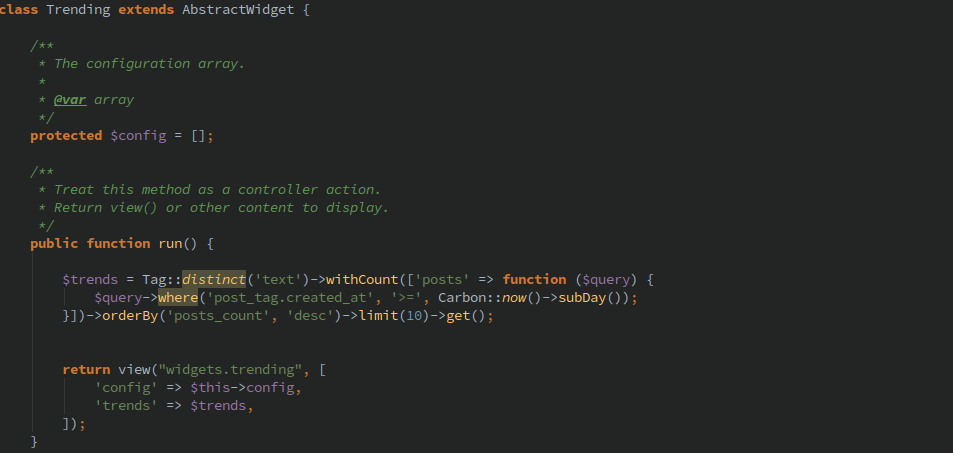
\includegraphics[width=\textwidth]{Images/Implementation/UI/Widgets/trending-class}
    \caption{Trending widget class}
    \label{fig:trending-class}
\end{figure}

\begin{figure}[H]
    \centering
    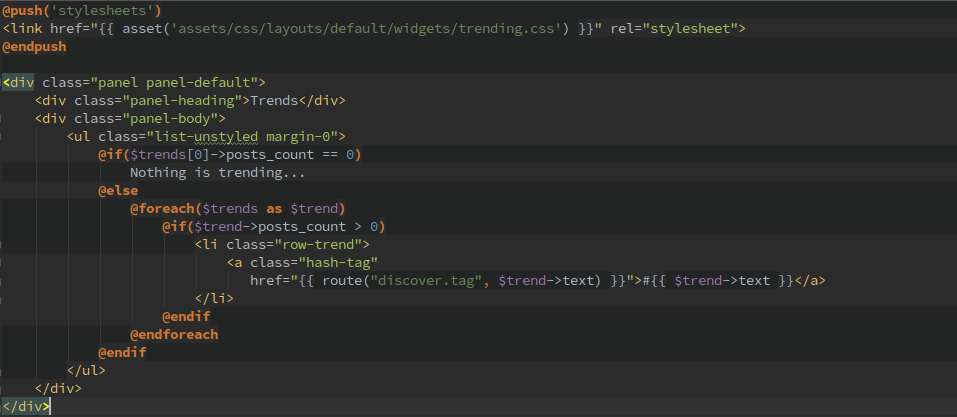
\includegraphics[width=\textwidth]{Images/Implementation/UI/Widgets/trending-blade}
    \caption{Trending widget view}
    \label{fig:trending-blade}
\end{figure}

\subsubsection{Recommendations}
Figure \ref{fig:RecommendationsWidget} shows the implementation of the recommendations widget. The widget allows the user to interact with the recommendations they receive. Interactions are limited to accepting or rejecting a recommendation. Additionally, users can navigate to the profile of the recommendation by clicking on their name. For both interaction types, the recommendation is removed from the widget. This ensures that the widget does not become bloated with recommendations the user has interacted with in the past, and the user is only shown recommendations they haven't responded to. Using jQuery it was possible to animate the removal of the recommendations from the widget. This provides the user with a visual cue of a successful interaction. Along with this animation, when a user accepts a recommendation the counter on the profile widget for the number of followers for the user is incremented. This again provides another visual cue to the user that their interaction has been successful.

\begin{figure}[H]
\centering
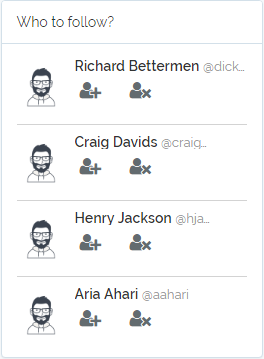
\includegraphics[height=3in]{Images/Implementation/RecommendationsWidget}
\caption{Recommendations widget}
\label{fig:RecommendationsWidget}
\end{figure}

In figure \ref{fig:UsersWidget} we can see the class for the user widget. This \textit{run()} function is responsible for collecting the user recommendations generated for the authorised user. Only recommendations the user has not responded to, denoted by a 0 in the database, are retrieved. Recommendations for a given user are fetched using the \textit{user\_recommendations} relation on the \emph{User} model.

\begin{figure}[H]
\centering
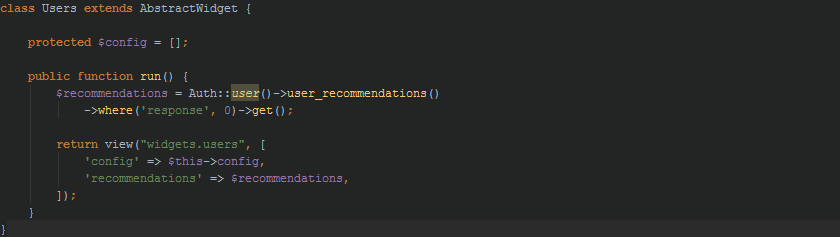
\includegraphics[width=1\textwidth]{Images/Implementation/UsersWidget}
\caption{User widget class}
\label{fig:UsersWidget}
\end{figure}

Figure \ref{fig:UserRecommendationsController} shows the controller created for the user recommendations. The controller handles interactions made with recommendations. The controller extends the \textit{FollowersController}, making it possible to use the custom HTTP request \textit{FollowRequest}, which is used when a request is made to follow a user. By extending this controller, the \textit{store()} function, which is called when the user accepts a recommendation, can log the follow request using its parent's \textit{store()} method, and then subsequently update the response to the request. The \textit{delete()} function is called when the user rejects one of the recommendations provided, and simply updates the response of the recommendation in the database.

\begin{figure}[H]
\centering
\includegraphics[width=1\textwidth]{Images/Implementation/UserRecommendationsController}
\caption{Users recommendations controller}
\label{fig:UserRecommendationsController}
\end{figure}